
A major experimental program is underway which seeks to measure
as of yet unknown properties associated with the change of flavor of neutrinos.
In particular, the neutrino mass hierarchy and charge-parity (CP) violating phase
of neutrinos still remain to be measured, with additional focuses on measuring
oscillation parameters with high precision and testing whether the current
three-flavor mixing paradigm is sufficient~\cite{Esteban:2020cvm, ParticleDataGroup:2020ssz}.
These goals introduce stringent requirements on the precision of current and future experiments.
High-intensity beams are required to produce the flux of neutrinos
 to be able to accumulate the necessary statistics.
Increased statistics place additional burden on the systematic uncertainties needed for the experimental program.

Two, billion dollar scale, next-generation experiments designed to meet these experimental constraints
are the Deep Underground Neutrino Experiment (DUNE)~\cite{Abi:2020wmh}
 and the Hyper-Kamiokande experiment (Hyper-K)~\cite{Hyper-Kamiokande:2018ofw}.
DUNE has a broad neutrino energy spectrum with a peak at a neutrino energy of $\approx$2.5 GeV,
but significant contributions between 0.1--10 GeV, over a 1295 km baseline. Hyper-K has a narrow
neutrino energy spectrum peaked at a neutrino energy of $\approx$0.6 GeV, with significant
contributions between 0.1--2 GeV, over a 295 km baseline. Despite their different energies and
baselines, both experiments sit at a similar L/E, so probe similar oscillation physics.
At the few-GeV energies of interest, neutrino interactions with nucleons have many available interaction channels,
 including quasielastic, resonant, and deep inelastic scattering~\cite{zeller12, hayato_review_2014, Mosel:2016cwa, Katori:2016yel, NuSTEC:2017hzk}.
All current and planned experiments use nuclear targets ($^{12}$C--$^{40}$Ar) as the
target material to increase the interaction rate, as well as to avoid serious experimental complications using elementary targets.
The use of nuclear targets significantly complicates the cross-section modeling issues and
associated systematics as intra-nuclear dynamics have a comparable energy scale to
the energy transfers in the neutrino interactions of interest.

A significant challenge impeding progress towards a consistent theoretical description of neutrino-nucleus interactions is the lack of data to benchmark parts of the calculation against. For example, neutrino quasielastic scattering ($\nu_{l} + n \rightarrow l^{-} + p$ or $\bar{\nu}_{l} + p \rightarrow l^{+} + n$) is the simplest of the relevant hard scattering processes, and dominates the neutrino cross section below \new{energies of} $\approx$1 GeV. However, modern experiments using nuclear targets are unable to measure it without significant nuclear effects~\cite{garvey_review_2014, NuSTEC:2017hzk}.
Neutrino cross-section models for quasielastic scattering (and other hard-scattering processes) have relied heavily on sparse data from the 1960--1980's from several bubble chamber experiments which used $H_{2}$ or $D_2$ targets~\cite{zeller12, ParticleDataGroup:2020ssz}.
The small neutrino cross section, and relatively weak (by modern standards) accelerator neutrino beams utilized by these early experiments, mean that the available quasielastic event sample on light targets amounts to a few thousand events~\cite{ANL_Barish_1977, BNL_Baker_1981}.
{\color{red} [We could consider adding some comments about pion electroproduction here]}

The sparse data from deuterium bubble chamber experiments do not constrain
 the axial form factor precisely.
The popular dipole axial form factor ansatz has a shape that
 is overconstrained by data, which results in an underestimated uncertainty.
Employing a model-independent $z$ expansion parameterization
 relaxes the strict shape requirements of the dipole and yields
 a more realistic uncertainty that is nearly an order of magnitude larger~\cite{Meyer:2016oeg}.
The axial radius, which is proportional to the slope of the form factor at $Q^2=0$,
 has a 50\% uncertainty when estimated from the deuterium scattering data,
 or about 35\% if deuterium scattering and muonic hydrogen are considered
 together~\cite{Hill:2017wgb}.
Ideally, the lack of precision in the axial form factor would
 be rectified by a modern neutrino scattering experiment.

Safety considerations make it unlikely that new high-statistics bubble chamber experiments \new{using}
hydrogen or deuterium will be deployed to fill this crucial gap,
so \new{experimentalists} are looking for other ways to access neutrino interactions
with elementary targets as a tool for disambiguating neutrino cross section modeling uncertainties.
One possibility is to use experiments with various hydrocarbon targets to subtract the carbon interaction contributions from
 the total hydrocarbon event rates, and produce ``on hydrogen'' measurements~\cite{PhysRevD.92.051302, PhysRevD.101.092003, Hamacher-Baumann:2020ogq, DUNE:2021tad}.
These ideas are promising, but typically rely on kinematic tricks that are only relevant for some channels, and it remains to be seen whether the \new{systematic uncertainty associated with modelling} the carbon subtraction can be adequately controlled. Such ideas may also be extended to other compound target materials with hydrogen or deuterium components.

\newasm{
In the absence of an updated scattering experiment on an elementary target,
 lattice QCD (LQCD) could provide the missing free nucleon amplitudes
 that are otherwise not known at the required precision.
Lattice computations access current insertions with a quark bilinear gamma structure.
For charged current quasielastic scattering of a neutrino with a free nucleon,
 the interaction is described by a $V-A$ weak interaction, with current contributions
\begin{align}
 \langle n | V^\mu | p \rangle
 &= \bar{u}_n \Big[
 F_1(q^2) \gamma^\mu +\frac{i}{2M} F_2(q^2) \sigma^{\mu\nu} q_\nu
 \Big] u_p,
 \nonumber\\
 \langle n | A^\mu | p \rangle
 &= \bar{u}_n \Big[
 F_A(q^2) \gamma^\mu \gamma_5 +\frac{1}{M} F_P(q^2) q^\mu \gamma_5
 \Big] u_p,
\end{align}
 with $Q^2 = -q^2$.
Existing calculations from LQCD extend up to a range of $Q^2 \lesssim 1~{\rm GeV}^2$,
 which is ideal for the neutrino interactions at the ${\rm GeV}$ energy scale.
}

\newasm{
The vector form factors, $F_1$ and $F_2$,
 are precisely estimated from electron-proton scattering data,
 up to a tension in existing parameterizations of the proton magnetic form factor
 shown in Fig.~\ref{fig:protonmagneticff}.
The tension is significant over all $Q^2 > 0$, at the level of several percent,
 including significant disagreement in the slope of the form factor at $Q^2 = 0$.
Of the nucleon form factor calculations from lattice QCD,
 the vector form factors are also the most mature,
 exhibiting no obvious tensions with experimental determinations
 of the vector form factors at the level of the lattice precision.
\textcolor{red}{[what percent precision?]}
A percent level calculation of the form factor $Q^2$ behavior
 or a direct calculation of the slope of the magnetic form factor
 would provide useful insight about this tension or could discriminate
 between the two parameterizations.
}

\new{
Fortunately, lattice QCD provides a theoretical alternative for predicting the free nucleon amplitudes directly from the Standard Model (SM) of particle physics, with systematically improvable theoretical uncertainties.}
%In the absence of an updated scattering experiment on an elementary target, lattice QCD (LQCD) could provide the missing free nucleon amplitudes that are otherwise not known at the required precision.
\new{The nucleon quasi-elastic form factor can be computed with a few-${\rm GeV}^2$ reach in momentum transfer and relatively small uncertainty.}
A tension in the neutron magnetic form factor parameterization, which is roughly half the size of the total axial form factor uncertainty, can be resolved with a similar LQCD calculation.
\new{Building upon these critical benchmark quantities,}
more challenging computations can provide information about nucleon
resonant and nonresonant contributions to axial matrix elements,
such as the $\Delta$ or Roper resonance channels, \new{pion-production,}
inclusive contributions in the shallow inelastic scattering region,
or deep inelastic scattering parton distribution functions.

\new{Given the present state of the field, in this review, we focus on elastic single-nucleon amplitudes, in which we anticipate the LQCD results will become impactful for the experimental programs in the next year or two.
For example, Figure~\ref{fig:protonmagneticff} demonstrates the current tension in the determination of the proton magnetic form factor.
Two different parameterizations of the form factor, normalized by the dipole are displayed.
The Bradford, Bodek, Budd and Arrington parameterization from Neutrino-Nucleus Interaction 2005 Workshop (BBBA05)~\cite{Bradford:2006yz} are displayed as the lower (blue) band with a solid mean value.
A more recent z-expansion parameterization from Borah {\it et al.}~\cite{Borah:2020gte} is displayed by the upper (black) band with a dashed mean value.
Of note, even the sign of the slope of the form factor is not determined.
}
%------------------------------------------------------------------------------
% proton magnetic FF
\begin{figure}[hbt!]
 \centering
 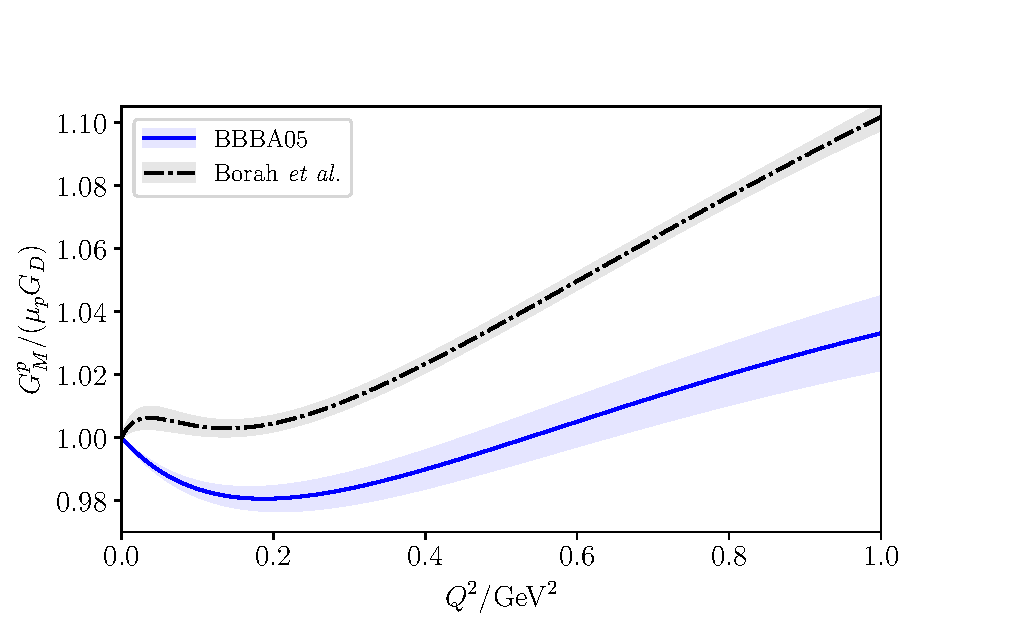
\includegraphics[width=0.75\textwidth]{plots/proton_magnetic-standalone.pdf}
\caption{
Proton magnetic form factor normalized by a reference dipole ansatz
with a dipole mass of $0.84~{\rm GeV}$.
The proton-only fit to a $z$ expansion by Borah {\it et al.}~\cite{Borah:2020gte}
and the BBBA05 parameterization~\cite{Bradford:2006yz} are shown.
\label{fig:protonmagneticff}
}
\end{figure}
%------------------------------------------------------------------------------



\newasm{
The nucleon axial form factor has had a much more complicated past
 than the vector form factors in lattice QCD.
The axial charge, the value of the axial form factor at $Q^2=0$,
 is a key benchmark for lattice QCD and is precisely known
 from neutron decay experiments.
LQCD calculations of the axial charge have historically been low compared
 to experiment, and the discrepancy has been the topic of some controversy.
As treatment of systematics have become more sophisticated,
 modern calculations of the axial charge have finally started to come into
 agreement with the experimental value at the percent level.
}

\newasm{
Armed with the newfound confidence in the control of systematics for the axial charge,
 more emphasis is now being put into the form factor at nonzero momentum transfer.
One extremely striking feature of lattice calculations is the strong preference for a slower
 fall off of the form factor with increasing $Q^2$ than predicted by experiment.
This preference is consistently reproduced by several lattice collaborations using
 independent computation methods, lending more credence to the result.
When integrated over the full range of $Q^2$ to compute the nucleon cross section,
 this translates to an enhancement in the free nucleon cross section as large as $30-40\%$
 over neutrino energies greater than $1~{\rm GeV}$.
In addition, the precision on the axial form factor uncertainty from lattice QCD
 is small enough to be sensitive to the tension between vector form factor parameterizations.
}

\newasm{
The aformentioned situation with nucleon form factors
 is depicted in Fig.~\ref{fig:nucleonxsec}.
The black dot-dashed curve is the default case,
 which uses the $z$ expansion parameterizations of the vector and axial
 form factors from Refs.~\cite{Borah:2020gte}~and~\cite{Meyer:2016oeg}, respectively.
The green band shows the uncertainty obtained from the axial form factor alone,
 and the gray band from the (much smaller) vector form factor uncertainty by itself.
The blue solid curve substitutes the vector form factors of the default choice
 with the BBBA05 parameterization~\cite{Bradford:2006yz},
 taking the uncorrelated uncertainty from the BBBA05 vector form factors only.
The observed tension between the black and blue bands is the result of the
 tension between proton magnetic form factor parameterizations.
The red dotted curve instead substitutes the axial form factor of the default
 with a parameterization obtained from lattice QCD and its uncertainty.
The size of the red band with respect to the green band demonstrates
 the uncertainty reduction from replacing the deuterium scattering
 axial form factor with one obtained from LQCD,
 and the significant change in normalization is due to the slower fall off
 of the axial form factor.
Additionally, the size of the red band demonstrates the relevance
 of the tension in vector form factors, characterized by the difference
 between the black and blue curves.
}

The relevance of this tension to the neutrino program can be understood from Figures~\ref{fig:nucleonxsec}.

%------------------------------------------------------------------------------
% nu-N cross section
\begin{figure}[hbt!]
 \centering
 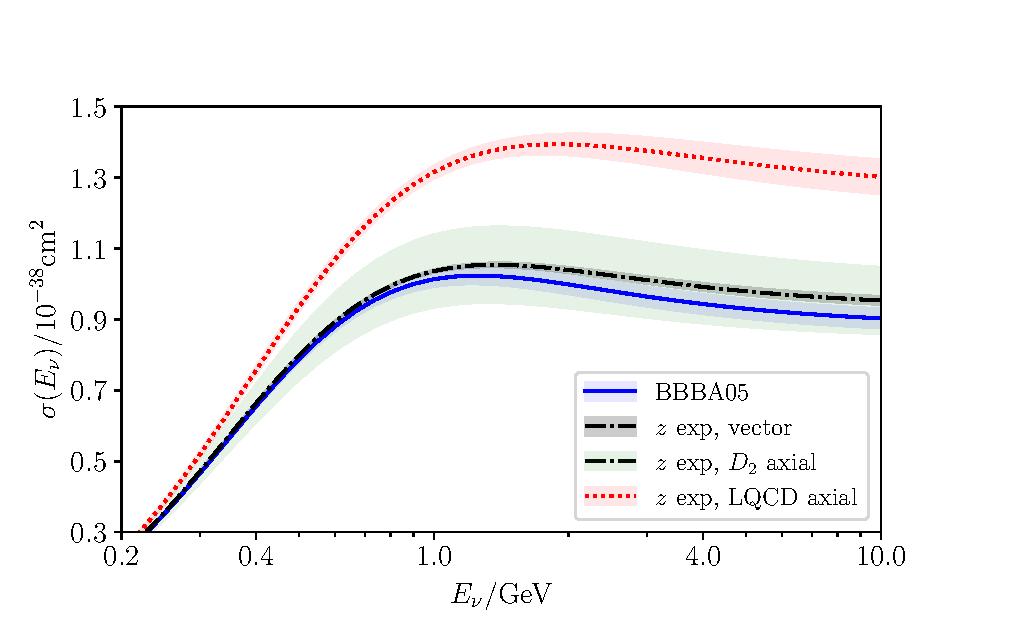
\includegraphics[width=0.75\textwidth]{plots/xsec_comparison-standalone.pdf}
\caption{
 Neutrino cross sections on a free neutron, with their uncertainty bands,
 for various choices of parameterization.
 The curves labeled ``BBBA05'' (blue solid line, Ref.~\cite{Bradford:2006yz})
 and ``$z$ exp, vector'' (black dot-dashed line, Ref.~\cite{Borah:2020gte}) use the
 $z$ expansion axial form factor from Ref.~\cite{Meyer:2016oeg},
 with only the uncertainty from the vector form factors plotted
 to highlight the tension between the parameterizations shown in Fig.~\ref{fig:protonmagneticff}.
 The same form factor parameterizations are used for both ``$z$ exp, vector'' and
 ``$z$ exp, $D_{2}$ axial'' (green dot-dashed line)
 but in the latter case the uncertainty band is taken only from
 the axial form factor rather than only from the vector form factor.
 The red dotted line labeled ``$z$ exp, LQCD axial'' is parameterized by
 the vector form factors of Ref.~\cite{Borah:2020gte} with no uncertainty
 and the axial form factor with its uncertainty taken from LQCD.
 \label{fig:nucleonxsec}
}
\end{figure}

\newasm{
So far, the focus of this manuscript has been on the charged-current
 quasielastic form factors, which are the easiest target for lattice QCD
 efforts and most relevant to the next-generation neutrino oscillation program.
Of these, the axial form factor has gotten the most attention from lattice collaborations
 and is the focus of the material in Sec.~\ref{sec:lqcd}.
The phenomenological impact of the axial form factor obtained from lattice QCD
 is given in more detail in Sec.~\ref{sec:impact}.
}

\newasm{
Similar calculations could also access the isoscalar form factors of the nucleon,
 which apply to neutral current scattering amplitudes,
 although the precision obtained from these calculations is more limited
 due to the sensitivity of the measurement to the background gauge fields
 in the lattice gauge configurations.
More challenging computations could provide information about nucleon
 resonant and nonresonant contributions to axial matrix elements,
 such as the $\Delta$ or Roper resonance channels,
 inclusive contributions in the shallow inelastic scattering region,
 or deep inelastic scattering parton distribution functions.
Some applications of lattice QCD to other interaction mechanisms
 are outlined in Sec.~\ref{sec:future}.
}

\begin{description}
\item[first $z$ exp vector form factor] \cite{Ye:2017gyb}
 - does not use constraints from muonic hydrogen, many more fit parameters
\item[Vector form factor tensions] \cite{Borah:2020gte}
\item[Muonic hydrogen review] \cite{Hill:2017wgb}
\end{description}

\textcolor{red}{[Most focus on axial, but vector is important too]}
